\documentclass[11pt, a4paper]{article}
\usepackage[margin=2.4cm]{geometry}
\usepackage[T1]{fontenc}
\usepackage{lmodern}          % Type 1 vector fonts
\usepackage{cmap}             % ToUnicode CMap -> copyable text and accents
\usepackage[utf8]{inputenc}
\usepackage[english]{babel}
\usepackage{amsmath, amssymb, amsthm}
\usepackage{bm}
\usepackage{mathtools}
\usepackage{enumitem}
\usepackage{booktabs}
\usepackage{array}
\usepackage{xcolor}
\usepackage{titlesec}
\usepackage{parskip}
\usepackage{hyperref}
\usepackage{fancyhdr}
\usepackage{tcolorbox}
\usepackage{graphicx}
\usepackage{caption}
\tcbuselibrary{skins, breakable}

\definecolor{darkblue}{RGB}{15,55,115}
\definecolor{midblue}{RGB}{30,100,180}
\definecolor{theorybg}{RGB}{245,250,255}
\definecolor{questionbg}{RGB}{255,252,240}
\definecolor{evencolor}{RGB}{60,0,100}
\definecolor{rubricbg}{RGB}{248,246,252}
\definecolor{planbg}{RGB}{246,252,247}
\definecolor{plancolor}{RGB}{20,95,55}
\definecolor{trapbg}{RGB}{255,247,245}
\definecolor{trapcolor}{RGB}{150,35,35}

\hypersetup{colorlinks=true, linkcolor=darkblue, urlcolor=midblue,
  pdftitle={Solutions --- Problem Set 6 --- Macroeconomics I MPE Insper},
  pdfauthor={Macroeconomia I --- MPE Insper 2026/T3}}

\setlength{\headheight}{14pt}
\pagestyle{fancy}
\fancyhf{}
\renewcommand{\headrulewidth}{0.4pt}
\fancyhead[L]{\small\textcolor{darkblue}{\textit{Macroeconomia I --- MPE Insper --- 2026/T3}}}
\fancyhead[R]{\small\textcolor{darkblue}{\thepage}}
\fancyfoot[C]{\small\textcolor{gray}{Solutions --- Problem Set 6}}

\titleformat{\section}[block]
  {\large\bfseries\color{darkblue}}{}{0pt}{}
  [\vspace{2pt}\color{darkblue}\rule{\textwidth}{1.5pt}\vspace{4pt}]

\tcbset{
  theorybox/.style={
    enhanced, breakable, colback=theorybg, colframe=darkblue,
    fonttitle=\bfseries\small, coltitle=white, boxrule=0.5pt, arc=3pt,
    left=6pt, right=6pt, top=4pt, bottom=4pt,
  },
  questionbox/.style={
    enhanced, breakable, colback=questionbg, colframe=gray!60,
    fonttitle=\bfseries\small, coltitle=black, boxrule=0.4pt, arc=2pt,
    left=6pt, right=6pt, top=4pt, bottom=4pt, title={\textit{Question}},
  },
  rubricbox/.style={
    enhanced, breakable, colback=rubricbg, colframe=evencolor!70,
    fonttitle=\bfseries\small, coltitle=white, boxrule=0.4pt, arc=2pt,
    left=6pt, right=6pt, top=4pt, bottom=4pt, title={Where the marks are},
  },
  planbox/.style={
    enhanced, breakable, colback=planbg, colframe=plancolor,
    fonttitle=\bfseries\small, coltitle=white, boxrule=0.5pt, arc=3pt,
    left=6pt, right=6pt, top=4pt, bottom=4pt,
  },
  trapbox/.style={
    enhanced, breakable, colback=trapbg, colframe=trapcolor!75,
    fonttitle=\bfseries\small, coltitle=white, boxrule=0.4pt, arc=2pt,
    left=6pt, right=6pt, top=4pt, bottom=4pt,
  },
}

\newcommand{\passo}[1]{\medskip\noindent\textbf{#1}\par\nobreak}
\newcommand{\intuicao}[1]{%
  \medskip\noindent\textcolor{midblue}{\textbf{Economic reading.}} #1\par}
\newcommand{\resp}[1]{%
  \ifmmode {\color{darkblue}#1}\else\textcolor{darkblue}{\textbf{#1}}\fi}
\newcommand{\stst}{^{\ast}}
\newcommand{\MRS}{\mathrm{MRS}}
\newcommand{\MRT}{\mathrm{MRT}}
\newcommand{\Kb}{\bar K}
\newcommand{\pb}{\bar p}
\newcommand{\Ms}{M^{S}}
\newcommand{\md}{m^{D}}
\newcommand{\Nst}{N^{\ast}}

\setlist[enumerate,1]{label=(\alph*), itemsep=6pt, parsep=2pt, leftmargin=1.6em}
\setlist[itemize,1]{itemsep=3pt, parsep=1pt, leftmargin=1.3em, topsep=3pt}

\begin{document}

%======================================================================
\begin{center}
{\LARGE\bfseries\color{darkblue} Solutions --- Problem Set 6\par}
\vspace{4pt}
{\large MACROECONOMIA 1 --- MPE Insper --- Prof.\ Pedro G.\ Duarte\par}
\vspace{2pt}
{\normalsize 2026, 3\textordmasculine{} trimestre \quad$\cdot$\quad Due: 21/09\par}
\vspace{2pt}
{\small Money and Inflation --- Kurlat (2020), ch.\ 10 and 11\par}
\end{center}
\vspace{6pt}

\begin{tcolorbox}[theorybox, title={How to read this document}]
\small
This file contains \textbf{both questions} (10 points). Question 1 asks what the quantity
equation \emph{is}; Question 2 puts the same equilibrium condition in growth rates, where it
finally does some work.

\smallskip
\textbf{What Question 1 is really about.} All four items circle one idea, and it is the idea
lecture 7 exists to install: \emph{the quantity equation is a container, not a theory}. Item
(a) empties the container. Item (b) fills it with one specific theory --- Baumol--Tobin ---
and shows that the theory immediately \textbf{contradicts} the assumption the crude quantity
theory needed, namely that velocity is a constant. Item (c) asks what the container can say
when the price level is nailed down, and the honest answer is \emph{almost nothing}, because
Kurlat ch.\ 11 assumes flexible prices throughout; the machinery to answer it is lecture 8's.
Item (d) shows that the very same equilibrium condition is read \textbf{left to right} when
the central bank sets $M$ and \textbf{right to left} when it sets $i$.

\smallskip
So the thread is: \emph{an identity has no causal content; a money-demand function supplies
it; and which variable is endogenous is a choice of monetary regime, not a fact about the
equation.}

\smallskip
Highlighted answers are in \resp{blue}. \textcolor{trapcolor}{\textbf{Red}} boxes are traps;
\textcolor{plancolor}{\textbf{green}} boxes are method. Page references are to the printed
pages of Kurlat (2020); the book's offset in this project is $0$, so printed page $=$ PDF
page.

\smallskip
\emph{Language.} Written in English, per the project's global output-language rule --- and in
any case the problem set itself is set in English. \emph{Notation.} Kurlat's: $\md(Y,i)$ for
real money demand, $p$ (lower case) for the price level, $\mu$ for money growth.
\end{tcolorbox}

\begin{center}
\small
\begin{tabular}{@{}lcl@{}}
\toprule
\textbf{Item} & \textbf{Weight} & \textbf{Basis in Kurlat} \\
\midrule
1(a) --- $MV=PY$ as an identity & $\approx1.25$ & \S11.2, pp.\ 208--215 \\
1(b) --- Baumol--Tobin and velocity & $\approx1.25$ & \S10.4, pp.\ 199--202; Ex.\ \textbf{10.5}, \textbf{11.1} \\
1(c) --- Fixed vs flexible $p$ & $\approx1.25$ & \S11.2, pp.\ 208--215 \\
1(d) --- Setting $M$ vs setting $i$ & $\approx1.25$ & \S10.2--10.3, pp.\ 192--199; \S11.2 \\
\midrule
2(a) --- $\pi=\mu-\eta g$ & $\approx1.7$ & \S11.2--11.3, pp.\ 208--218 \\
2(b) --- Targeting, $\eta=\tfrac12$ vs $\eta=1$ & $\approx1.7$ & \S10.4, pp.\ 199--202; \S11.3 \\
2(c) --- Falling trip cost, $\pi=\mu-\tfrac12(g+f)$ & $\approx1.6$ & \S10.4 + \S11.3 \\
\bottomrule
\end{tabular}
\end{center}

%======================================================================
\section{Question 1 \quad The quantity equation, money demand, and the monetary regime}
%======================================================================

\begin{tcolorbox}[planbox, title={Before writing anything: separate the three objects}]
\small
The question keeps three things in play that are easy to blur, and most lost marks come from
blurring them:
\begin{itemize}
\item \textbf{An identity} --- $MV=PY$. True by construction, for any data, in any model.
      Content: zero.
\item \textbf{A behavioural function} --- $\md(Y,i)$, with $\md_Y>0$ and $\md_i<0$. This is a
      \emph{theory}: it says what people choose to hold, and it is refutable.
\item \textbf{An equilibrium condition} --- $\Ms=p\,\md(Y,i)$. This says the two sides meet.
      It contains \emph{one} equation, so it can determine exactly \emph{one} endogenous
      variable, and which one that is depends on the policy regime (item (d)).
\end{itemize}
Every item below is an application of that three-way split.
\end{tcolorbox}

%----------------------------------------------------------------------
\subsection*{Item (a) --- why $MV=PY$ is an accounting identity and not a theory}
%----------------------------------------------------------------------

\passo{Step 1. $V$ is not measured; it is \emph{defined}.}
Nowhere in the construction of the equation is velocity observed. $P$ comes from a price
index, $Y$ from the national accounts, $M$ from a monetary aggregate. Velocity is then
obtained as the residual that makes the equation true:
\begin{equation}
V \;\equiv\; \frac{PY}{M}.
\label{eq:vdef}
\end{equation}
Substituting \eqref{eq:vdef} back into $MV=PY$ gives $M\cdot\frac{PY}{M}=PY$, i.e.\ $PY=PY$.

\resp{The equation is an identity because $V$ is defined residually: it is true by
construction for every economy, every period and every model, so it excludes nothing and
cannot be refuted by any data.} A statement that no observation could contradict carries no
information about the world.

\passo{Step 2. Counting equations and unknowns.}
There are four variables --- $M$, $V$, $p$, $Y$ --- and one equation. One equation cannot
determine four unknowns. It can at most determine \emph{one} of them once the other three are
given from outside. Any theory that claims to say what happens to $p$ after a change in $M$
must therefore bring in \textbf{three more restrictions} from elsewhere. It is not that the
identity is wrong; it is that it is \emph{empty until supplemented}.

\passo{Step 3. Does it tell us whether a change in $M$ causes a change in $p$, $Y$ or $V$?}

\resp{No. The identity is silent on both the \emph{direction} of causation and the
\emph{split} of the adjustment.} Concretely, write it in growth rates (this is the form the
lecture uses, and it makes the point visible):
\begin{equation}
g_M + g_V \;=\; \pi + g_Y .
\label{eq:growth}
\end{equation}
A 10\% rise in $M$ is consistent with \emph{every} one of the following, and the identity
cannot discriminate between them:
\begin{center}
\small
\begin{tabular}{@{}llp{6.9cm}@{}}
\toprule
\textbf{Adjustment} & \textbf{$g_M=10\%$ absorbed by} & \textbf{The world in which it happens} \\
\midrule
Pure inflation & $\pi=10\%$ & Classical: $V$ stable, $Y$ at full employment. \\
Pure output & $g_Y=10\%$ & Deep slump, idle capacity, prices stuck. \\
Pure velocity & $g_V=-10\%$ & Liquidity trap or a hoarding panic: the extra money is held, not spent. \\
Reverse causation & $g_V=-10\%$ & The central bank pegs $i$ and passively supplies whatever $M$ a higher $p$ and $Y$ call for --- here $p$ and $Y$ cause $M$, not the other way round. \\
\bottomrule
\end{tabular}
\end{center}

The last row is the decisive one, and it is worth saying explicitly: since $M$ appears in the
identity symmetrically with everything else, \resp{the identity is equally consistent with
money being \emph{endogenous}} --- which is exactly the regime discussed in item (d). No
amount of staring at $MV=PY$ can settle which regime an economy is in.

\passo{Step 4. What turns the identity into the Quantity Theory.}
Three assumptions, all of them substantive and all of them refutable:
\begin{enumerate}[label=(\roman*)]
\item \textbf{Velocity is stable}, or at least exogenous to $M$ --- so $g_V\approx0$. This is
      the step that promotes $V$ from residual to behavioural constant, and it is the step
      item (b) will show is \emph{false} under Baumol--Tobin.
\item \textbf{Output is determined by the real side} --- technology, capital, labour supply
      (the classical dichotomy, chs.\ 5--9). So $g_Y$ is fixed independently of $M$.
\item \textbf{The money supply is controlled by the central bank}, i.e.\ $M$ is exogenous ---
      which fixes the direction of causation by assumption, not by evidence.
\end{enumerate}
Only with all three does \eqref{eq:growth} collapse to $\pi \approx g_M - g_Y$ and license the
claim that inflation is a monetary phenomenon.

\intuicao{The identity is the \emph{budget constraint} of the aggregate payments system: it
says that the money stock, turned over $V$ times, must have financed the nominal transactions
that actually took place. Budget constraints never explain behaviour. The theory lives
entirely in the assumptions about what $V$ does, and $V$ is a \emph{behavioural} object ---
how often people choose to part with money --- disguised as an arithmetic one.}

\begin{tcolorbox}[trapbox, title={The trap: answering ``because money causes inflation''}]
\small
The item is not asking whether the quantity theory is empirically right. It is asking a
logical question: \emph{what does this equation, by itself, assert?} The answer is ``nothing
that could be false''. Any answer that defends or attacks the quantity theory without first
saying that $V$ is defined residually has missed the question. State the identity/theory
distinction first, then name the three assumptions, then --- if you like --- say that the
quantity theory is a good long-run description and a poor short-run one.
\end{tcolorbox}

%----------------------------------------------------------------------
\subsection*{Item (b) --- Baumol--Tobin: money demand, and what it says about velocity}
%----------------------------------------------------------------------

\begin{tcolorbox}[planbox, title={Build the square root; do not quote it}]
\small
The marks here are for deriving $\md=\sqrt{YF/2i}$ from the trip-cost problem and then
\textbf{inverting it into velocity}. Quoting the formula and stopping is a half answer,
because the item explicitly asks about velocity, and velocity is the bridge back to item (a).
\end{tcolorbox}

\passo{Step 1. The problem (Kurlat \S10.4, pp.\ 199--202).}
A household spends at a constant rate over the period, for a total real value $Y$. It keeps
its wealth in an interest-bearing account paying nominal rate $i$ and must convert it into
money to spend. Each conversion --- a ``trip to the bank'' --- costs a fixed real amount $F$,
independent of the amount withdrawn. Let $N$ be the number of trips.

\passo{Step 2. The two costs.}
With $N$ evenly spaced trips, each withdrawal is $Y/N$ in real terms and balances run down
linearly to zero before the next trip. Money holdings therefore trace a \textbf{sawtooth}
between $Y/N$ and $0$, so average real balances are
\begin{equation}
\md \;=\; \frac{Y}{2N}.
\label{eq:sawtooth}
\end{equation}
Holding money forgoes the nominal interest $i$ on those balances, and the $N$ trips cost $NF$.
The total real cost of the cash-management strategy is
\begin{equation}
\Phi(N) \;=\; \underbrace{i\,\frac{Y}{2N}}_{\text{interest forgone}} \;+\; \underbrace{NF}_{\text{trip costs}}.
\label{eq:cost}
\end{equation}
The trade-off is transparent: more trips economise on forgone interest but cost more in $F$.

\passo{Step 3. The optimum.}
\[
\Phi'(N) \;=\; -\,\frac{iY}{2N^{2}} + F \;=\; 0
\qquad\Longrightarrow\qquad
\resp{\Nst=\sqrt{\dfrac{iY}{2F}}},
\]
and $\Phi''(N)=iY/N^{3}>0$, so this is a minimum. Substituting $\Nst$ into
\eqref{eq:sawtooth}:
\begin{equation}
\md(Y,i) \;=\; \frac{Y}{2\Nst} \;=\; \frac{Y}{2}\sqrt{\frac{2F}{iY}}
\;=\; \resp{\sqrt{\frac{YF}{2i}}}.
\label{eq:bt}
\end{equation}
This is increasing in $Y$ and decreasing in $i$, as the question's $\md(Y,i)$ requires --- so
Baumol--Tobin is not an alternative to the framework of Equation~(2), it is a \emph{derivation
of it from optimisation}. Taking logs,
\[
\ln \md = \tfrac12\ln Y + \tfrac12 \ln F - \tfrac12\ln i - \tfrac12\ln 2,
\]
so the elasticities are read off directly:
\begin{equation}
\resp{\varepsilon_{\md,Y}=+\tfrac12,\qquad
\varepsilon_{\md,i}=-\tfrac12,\qquad
\varepsilon_{\md,F}=+\tfrac12 .}
\label{eq:elast}
\end{equation}

\passo{Step 4. Now the velocity implication --- what the item is actually asking.}
Combine \eqref{eq:vdef} with the equilibrium condition $M=p\,\md$. Then $V=PY/M=Y/\md$, and
substituting \eqref{eq:bt}:
\begin{equation}
V \;=\; \frac{Y}{\sqrt{YF/2i}} \;=\; \resp{\sqrt{\frac{2iY}{F}}}.
\label{eq:velocity}
\end{equation}
Reading the elasticities of \eqref{eq:velocity} off its logarithm:
\begin{equation}
\resp{\varepsilon_{V,i}=+\tfrac12,\qquad
\varepsilon_{V,Y}=+\tfrac12,\qquad
\varepsilon_{V,F}=-\tfrac12 .}
\end{equation}

\resp{The model therefore says velocity is \emph{not} a constant and \emph{not} a residual: it
is a behavioural variable, the reciprocal of real money demand per unit of income, and it is
systematically driven by the nominal interest rate, by the scale of transactions, and by the
technology of the payments system.} Three consequences, each of which is a mark:

\begin{itemize}
\item \textbf{$V$ rises with $i$.} High nominal interest makes money expensive to hold; people
      economise on balances, so each unit of money turns over more often. This is the single
      most damaging result for the crude quantity theory, because it makes $V$ move with
      exactly the variable monetary policy moves.
\item \textbf{$V$ rises with $Y$ --- there are economies of scale in cash management.} Since
      $\varepsilon_{\md,Y}=\tfrac12<1$, money demand grows \emph{less} than proportionally
      with income, so $V$ trends \emph{upward} as an economy grows even at constant $i$. The
      Cambridge equation, and the quantity theory built on it, implicitly assume
      $\varepsilon_{\md,Y}=1$ and hence a trendless $V$. \emph{(This is precisely the $\eta$
      of Question 2: Baumol--Tobin gives $\eta=\tfrac12$, Cambridge gives $\eta=1$.)}
\item \textbf{$V$ falls with $F$ --- velocity is a technology.} ATMs, debit cards and instant
      payment systems (Pix) all cut $F$; every such innovation raises $V$ permanently. So even
      the historical stability of $V$ cannot be assumed: it is hostage to the payments system.
      \emph{(This is Question 2(c): $\dot F/F=f<0$.)}
\end{itemize}

\begin{tcolorbox}[planbox, title={A clean way to see \eqref{eq:velocity}: velocity \emph{is} the trips}]
\small
Compare $\Nst=\sqrt{iY/2F}$ with $V=\sqrt{2iY/F}$: they differ by a factor of exactly $2$,
\[
\resp{V = 2\Nst .}
\]
That is not a coincidence. Each trip puts a lump of money into circulation that is then spent
down to zero, so over the period the stock $M$ finances $N$ full lumps --- but because the
\emph{average} balance is only half of each lump, the average stock turns over twice per trip.
Velocity is literally a count of how often the representative household goes to the bank. It
is a \textbf{behavioural frequency}, which is the whole point against item (a).

\smallskip
Two further identities worth keeping. At the optimum the two components of \eqref{eq:cost}
are \emph{equal}, each being $\sqrt{iYF/2}$ (this is the expression the slides quote as the
total trip cost, $\Nst F$), so total shoe-leather cost is $\Phi(\Nst)=\sqrt{2iYF}$; and
$\Phi(\Nst)=2\,i\,\md$, i.e.\ the resource cost of inflation is proportional to the product of
the nominal rate and real balances. That is the formal basis of the \textbf{Friedman rule}
($i=0$, so $\pi=-r$) in \S11.4.
\end{tcolorbox}

\begin{tcolorbox}[trapbox, title={The trap: stopping at $\sqrt{YF/2i}$}]
\small
The item says ``money demand \textbf{and} the velocity of money''. An answer that derives
\eqref{eq:bt} and says ``money demand falls with the interest rate'' has answered half the
question and, worse, has missed the punchline: \emph{Baumol--Tobin is a refutation of the
assumption that made the quantity equation into a theory in item (a).} Write $V=\sqrt{2iY/F}$
explicitly and say so.

\smallskip
Second trap: do not claim that Baumol--Tobin makes the quantity theory \emph{wrong}. It makes
the constant-$V$ shortcut wrong. The long-run link from money growth to inflation survives
intact --- it just needs $\eta$ in it, which is exactly Question 2's $\pi=\mu-\eta g$.
\end{tcolorbox}

%----------------------------------------------------------------------
\subsection*{Item (c) --- an increase in $\Ms$ with $p=\pb$ fixed, and then with $p$ flexible}
%----------------------------------------------------------------------

\passo{Step 1. What the equilibrium condition forces.}
Equation~(2) with the price level nailed at $\pb$ reads
\begin{equation}
\Ms \;=\; \pb\;\md(Y,i)
\qquad\Longleftrightarrow\qquad
\md(Y,i) \;=\; \frac{\Ms}{\pb}.
\label{eq:fixedp}
\end{equation}
An exogenous rise in $\Ms$ raises the target $\Ms/\pb$ \textbf{one for one}, because $\pb$
cannot absorb any of it. Real balances in circulation have risen, and the public must be
induced to \emph{want} to hold them. Since $\md_Y>0$ and $\md_i<0$:
\[
\resp{\text{real income must rise, or the nominal interest rate must fall, or both:}\qquad
Y\uparrow \ \text{ and/or } \ i\downarrow .}
\]
Totally differentiating \eqref{eq:fixedp} makes the trade-off explicit:
\begin{equation}
\md_Y\,dY + \md_i\,di \;=\; \frac{d\Ms}{\pb},
\qquad\text{so along the locus}\qquad
\left.\frac{dY}{di}\right|_{\text{money mkt}} = -\frac{\md_i}{\md_Y} > 0 .
\label{eq:lm}
\end{equation}

\passo{Step 2. The first honest point: \eqref{eq:fixedp} is \emph{one} equation in \emph{two} unknowns.}
\resp{The money market alone cannot determine the split between $Y$ and $i$.} It delivers a
whole locus of $(Y,i)$ pairs --- \eqref{eq:lm} is an upward-sloping curve in $(Y,i)$ space,
shifted right by the money injection --- and a second relation is needed to pick a point on
it. That second relation would have to come from the goods market. Kurlat ch.\ 11 does not
supply one, because it never needs one: with flexible prices $Y$ is already pinned by the real
block.

\passo{Step 3. Closing it the only way ch.\ 11 allows, and finding the tension.}
If we keep the classical assumption that $Y$ is determined by the real block --- technology,
capital, labour supply --- then $Y=\bar Y$ even here, and the entire adjustment falls on the
interest rate: $i$ must fall until $\md(\bar Y,i)=\Ms/\pb$. Under Baumol--Tobin \eqref{eq:bt}
this is quantitative: since $\varepsilon_{\md,i}=-\tfrac12$,
\[
\hat{\imath} \;=\; -\,2\,\hat{\md} \;=\; -\,2\,\widehat{\Ms},
\]
so a 1\% rise in the money supply requires a \textbf{2\% fall} in the nominal rate --- a very
large move, and one that quickly runs into the bound $i\ge0$.

But now apply the Fisher equation, $i=r+\pi^{e}$. With the price level fixed at $\pb$ and
expected to stay there, $\pi^{e}=0$, so a fall in $i$ \emph{is} a fall in the real rate $r$.
And the real block of chs.\ 6 and 9 already pinned $r$ --- to the household's impatience and
the marginal product of capital. \resp{Fixing $p$ therefore over-determines the model: the
money market demands a lower $r$, the real block insists $r$ is unchanged.} Something has to
give, and nothing in ch.\ 11 is allowed to give.

\passo{Step 4. Is there a clear mechanism for how this change occurs?}

\resp{No --- and saying so is the answer.} Chapter 11 has no channel from a lower nominal
interest rate to higher output. There is no investment demand schedule responding to $r$
(investment is ch.\ 8, outside this course), no sticky-price firm choosing how much to
produce, no aggregate demand relation at all. The chapter's entire adjustment mechanism
\emph{is} the price level: when people find themselves holding more money than they want, they
try to spend it, and in a flexible-price world the attempt bids $p$ up until real balances are
back where they were. \textbf{Take that mechanism away by assumption and the model is mute.}

What the fixed-price assumption is really doing is asserting the conclusion of a model the
course has not yet built. \resp{Supplying the missing mechanism --- why prices are sticky, and
how an excess supply of money then raises output rather than prices --- is the job of lecture
8 and the AD--AS material.} The correct answer names the gap instead of papering over it.

\intuicao{Item (c) is the seam of the whole course. Lectures 5--7 build a world in which money
is a veil; lectures 8--9 tear one hole in it. This item stands exactly on the tear and asks
you to notice that you are standing on it.}

\passo{Step 5. Do the answers change if prices are flexible? Yes --- completely.}
With $p$ free, the classical dichotomy is restored and the money market determines the one
variable it is capable of determining, namely $p$:
\begin{equation}
p \;=\; \frac{\Ms}{\md(\bar Y,\bar\imath)} .
\label{eq:pflex}
\end{equation}
Here $\bar Y$ comes from the real block and $\bar\imath=\bar r+\pi^{e}$ with $\bar r$ also
from the real block. Both are \textbf{independent of $\Ms$}. Hence a one-time increase in the
money supply leaves $Y$, $r$, $i$ and real balances $M/p$ all unchanged, and
\[
\resp{\frac{dp}{p} \;=\; \frac{d\Ms}{\Ms}\qquad\text{--- the price level rises exactly in
proportion. This is the \textbf{neutrality of money}.}}
\]
Note what has switched: under $p=\pb$ the money market was asked to determine \emph{real}
variables and could not do it alone; under flexible $p$ it determines a purely \emph{nominal}
variable and does it on its own. That is precisely the classical dichotomy.

\begin{tcolorbox}[trapbox, title={Neutrality is not superneutrality --- the second experiment}]
\small
Everything in Step 5 concerns a one-time jump in the \emph{level} of $\Ms$. A permanent
increase in its \emph{growth rate}, $\mu\to\mu'>\mu$, is a different experiment and the answer
is different:
\begin{enumerate}[label=\arabic*.]
\item Higher $\mu$ raises expected inflation, $\pi^{e}\uparrow$ (Question 2: $\pi=\mu-\eta g$).
\item By Fisher, $i=\bar r+\pi^{e}$ rises --- the \emph{real} rate is untouched, but the
      nominal one is not.
\item A higher $i$ \emph{lowers} desired real balances, $\md(\bar Y,i)\downarrow$ (by
      $\tfrac12$\% for each 1\% rise in $i$, under Baumol--Tobin).
\item By \eqref{eq:pflex}, $p$ must therefore \textbf{jump on announcement} --- more than
      proportionally --- \emph{and then} grow faster.
\end{enumerate}
So money is neutral (a level change does nothing real) but \textbf{not superneutral} (a growth
change lowers real balances, raises $\Nst$, and raises the shoe-leather cost $\sqrt{2iYF}$ of
item (b)). Writing ``money is neutral, therefore nothing real happens'' without this
distinction is the classic lost mark in this chapter.
\end{tcolorbox}

%----------------------------------------------------------------------
\subsection*{Item (d) --- reading the equilibrium under the two monetary regimes}
%----------------------------------------------------------------------

The equation does not change. \resp{What changes is which symbol is the unknown --- and
therefore in which direction the equation is read.}

\passo{Regime 1. The central bank controls the money supply.}
Set $\Ms=\bar M$. Then the left-hand side of the equilibrium condition is a number and
\[
\bar M \;=\; p\,\md(Y,i)\quad\text{is solved for}\quad \resp{i}\ \text{(short run, $p$ given)}
\quad\text{or for}\quad \resp{p}\ \text{(long run, $i$ given by the real block)}.
\]
Graphically, in $(M/p,\,i)$ space money supply is a \textbf{vertical line} at $\bar M/p$, and
the interest rate is the price that clears the market, found where the downward-sloping
$\md(Y,i)$ crosses it. The reading is \textbf{left to right}: the quantity is the instrument,
the interest rate is the outcome.

Two consequences follow, and both are worth stating:
\begin{itemize}
\item \textbf{The bank controls $M$ only indirectly.} What it actually sets is the monetary
      base $B$, through open-market operations, the discount window and reserve requirements
      (\S10.3, pp.\ 194--199). The broad aggregate is $M=m\cdot B$ with
      $m=\frac{1+cr}{rr+cr}$, and $m$ is a \emph{behavioural} object depending on banks'
      reserve choices and the public's currency ratio. It is not a constant: it collapses in a
      crisis, as it did in the United States in late 2008, when banks absorbed the base
      expansion as excess reserves and $M$ barely moved.
\item \textbf{Any shift in money demand shows up as interest-rate volatility.} With supply
      vertical, a shock to $\md$ --- a fall in $F$, a payments innovation, a precautionary
      scramble --- moves $i$ along the supply line.
\end{itemize}

\passo{Regime 2. The central bank controls the nominal interest rate.}
Now set $i=\bar\imath$ and the same equation is read \textbf{right to left}:
\begin{equation}
\resp{\Ms \;=\; p\,\md(Y,\bar\imath)} \qquad \text{now \emph{determines} } \Ms .
\end{equation}
Graphically, money supply is a \textbf{horizontal line} at $\bar\imath$: the bank stands ready
to buy or sell government bonds in unlimited quantity at that rate, and therefore supplies
whatever quantity of money the public wishes to hold at $\bar\imath$. \resp{The money stock
becomes \emph{endogenous} --- a residual, demand-determined, no longer ``chosen'' by the bank
in any meaningful sense.} Deviations of $\md$ are absorbed by quantity rather than by price,
so $i$ is stable and $M$ is volatile --- the mirror image of Regime 1.

This is what essentially every modern central bank does: the Banco Central announces the
Selic, the Fed a federal funds target, and the corresponding monetary aggregate is whatever it
turns out to be.

\passo{Why the two regimes are not the same thing.}
\begin{itemize}
\item \textbf{They coincide only under perfect knowledge of $\md$.} If the bank knew
      $\md(\cdot)$ exactly, picking $\bar M$ and picking the $\bar\imath$ it implies would be
      the same act. The regimes differ precisely because $\md$ is \emph{unstable} --- and item
      (b) explained why it must be: real money demand depends on the payments technology $F$,
      which drifts. \resp{An unstable $\md$ is the reason interest-rate control won:} under a
      quantity rule every shift in $\md$ contaminates $i$ and hence the real economy, whereas
      under a rate peg it is absorbed silently by $M$.
\item \textbf{The long-run quantity theory survives either way.} Pegging $i$ does not exempt
      the bank from the arithmetic of item (a). The $M$ it passively supplies still has a
      growth rate, and that growth rate still delivers $\pi=\mu-\eta g$. Controlling $i$
      changes \emph{who} chooses $\mu$ --- it becomes the by-product of the chosen rate path
      --- not whether $\mu$ matters.
\item \textbf{A rate peg needs a nominal anchor.} If the bank fixed $\bar\imath$ forever and
      responded to nothing, \eqref{eq:pflex} would pin real balances but leave the price level
      free: nothing in the system would say what $p$ is. This is why real inflation-targeting
      regimes set $i$ as a \emph{rule responding to inflation} rather than as a constant.
      Kurlat ch.\ 11 does not develop this; flag it as the reason the two regimes are not
      symmetric in the long run, and leave it there.
\end{itemize}

\intuicao{One equilibrium condition, one degree of freedom. The bank may choose the point on
the money-demand curve by naming its horizontal coordinate ($M$) or its vertical coordinate
($i$), but it cannot name both, and it cannot move the curve. Monetary ``control'' is the
choice of which coordinate to announce.}

\begin{tcolorbox}[rubricbox]
\small
\begin{itemize}
\item \textbf{(a)} $V\equiv PY/M$ is defined residually $\Rightarrow$ true by construction,
      unfalsifiable; one equation, four unknowns; explicitly \emph{no} causal content, in
      either direction or in the split; name the three assumptions (stable $V$, real-side
      $Y$, exogenous $M$) that make it the quantity theory.
\item \textbf{(b)} Derive $\Nst=\sqrt{iY/2F}$ and $\md=\sqrt{YF/2i}$ from
      $\Phi(N)=iY/2N+NF$; elasticities $+\tfrac12$, $-\tfrac12$. \textbf{Then invert:}
      $V=\sqrt{2iY/F}=2\Nst$. Velocity is behavioural, rises with $i$ and with $Y$, falls with
      $F$ --- so the constant-$V$ assumption of (a) is exactly what Baumol--Tobin denies.
\item \textbf{(c)} $\md(Y,i)=\Ms/\pb$ $\Rightarrow$ $Y\uparrow$ and/or $i\downarrow$; one
      equation, two unknowns, so the split is undetermined; if $Y=\bar Y$ classically then
      $\hat{\imath}=-2\widehat{\Ms}$, and Fisher puts that in conflict with the real block's
      $r$; \textbf{no mechanism exists in ch.\ 11} --- that is lecture 8. With flexible $p$:
      dichotomy restored, $p$ moves proportionally, money neutral. Add: neutral but not
      superneutral.
\item \textbf{(d)} Same equation, opposite reading. $\bar M$ $\Rightarrow$ vertical supply,
      $i$ endogenous, $M=mB$ with $m$ unstable (2008). $\bar\imath$ $\Rightarrow$ horizontal
      supply, $M$ endogenous and demand-determined. Equivalent only if $\md$ is known; the
      instability of $\md$ (item (b)'s $F$) is why rate control is the modern practice; the
      long-run $\pi=\mu-\eta g$ binds either way.
\end{itemize}
\end{tcolorbox}

%======================================================================
\section{Question 2 \quad Steady-state inflation: $\pi=\mu-\eta g$}
%======================================================================

\begin{tcolorbox}[planbox, title={What changes from Question 1}]
\small
Question 1 stayed at a point in time. Question 2 puts the \emph{same} equilibrium condition
$\Ms=p\,\md(Y,i)$ in \textbf{growth rates}, which is the only step that matters here: every
item is one log-differentiation away from the answer. The single trick is that a constant
nominal interest rate kills the $i$ term, so real money demand grows only through $Y$ --- and
through $F$, once item (c) lets the payments technology move.
\end{tcolorbox}

%----------------------------------------------------------------------
\subsection*{Item (a) --- deriving $\pi=\mu-\eta g$ from the equilibrium condition}
%----------------------------------------------------------------------

\passo{Step 1. Take logs of the equilibrium condition.}
The money market clears at every date, so \eqref{eq:pflex} holds as an identity in time:
\begin{equation}
\Ms_t \;=\; p_t\,\md(Y_t,i_t)
\qquad\Longrightarrow\qquad
\ln \Ms_t \;=\; \ln p_t + \ln \md(Y_t,i_t).
\label{eq:logeq}
\end{equation}
Logs are the right move because the question is about \emph{rates}, and the rate of change of
a variable is the time derivative of its log: $\dot x/x = \mathrm{d}\ln x/\mathrm{d}t$.

\passo{Step 2. Differentiate with respect to time.}
Differentiating \eqref{eq:logeq}, and using the chain rule on $\md(Y_t,i_t)$,
\begin{equation}
\underbrace{\frac{\dot \Ms}{\Ms}}_{=\;\mu}
\;=\;
\underbrace{\frac{\dot p}{p}}_{=\;\pi}
\;+\;
\underbrace{\frac{\partial \md}{\partial Y}\frac{Y}{\md}}_{=\;\eta}\,
\underbrace{\frac{\dot Y}{Y}}_{=\;g}
\;+\;
\frac{\partial \md}{\partial i}\frac{i}{\md}\,\frac{\dot\imath}{i}.
\label{eq:growth}
\end{equation}
The last term is where the steady-state assumption bites. \resp{The nominal interest rate is
constant, so $\dot\imath=0$ and the interest term vanishes} --- \emph{regardless} of how large
the interest elasticity is. Nothing had to be assumed about the level of $i$, only that it is
not moving.

\passo{Step 3. Solve for inflation.}
With $\dot\imath=0$, \eqref{eq:growth} collapses to $\mu=\pi+\eta g$, that is
\begin{equation}
\boxed{\;\resp{\pi \;=\; \mu-\eta g\;}}
\label{eq:piug}
\end{equation}
\checkmark\ Dimension check: all four objects are growth rates (per unit of time), and $\eta$
is a pure number, so the equation is homogeneous.

\intuicao{Inflation is the gap between how fast the \emph{supply} of money grows and how fast
the economy's \emph{demand} for real balances grows. Real money demand grows at $\eta g$:
output growth $g$ pulls money demand up, but only with elasticity $\eta$. Whatever money is
supplied over and above what people want to hold has nowhere to go but into the price level.
Money growth is not inflationary \emph{per se} --- money growth in excess of real money demand
growth is.}

\begin{tcolorbox}[theorybox, title={How this contains the crude quantity theory as a special case}]
\small
Set $\eta=1$ and \eqref{eq:piug} becomes $\pi=\mu-g$: the textbook quantity-theory formula,
equivalently $\mu = \pi + g$ with velocity constant. Indeed with $V$ constant, taking logs of
$MV=PY$ and differentiating gives $\mu+\hat V=\pi+g$ with $\hat V=0$. So $\eta=1$ \emph{is}
the constant-velocity assumption, restated as a property of money demand. More generally,
\begin{equation}
\hat V \;=\; \widehat{(Y/\md)} \;=\; g-\eta g \;=\; (1-\eta)\,g ,
\label{eq:vhat}
\end{equation}
which is the exact bridge back to Question 1(b): velocity trends up ($\hat V>0$) precisely
when $\eta<1$, i.e.\ precisely when there are economies of scale in cash management. The three
cases are worth memorising: $\eta<1 \Rightarrow \hat V>0$; $\eta=1 \Rightarrow \hat V=0$
(Cambridge, constant velocity); $\eta>1 \Rightarrow \hat V<0$.
\end{tcolorbox}

\begin{tcolorbox}[trapbox, title={Two traps in one line of algebra}]
\small
\textbf{(i) Do not drop the interest term by assuming $\md_i=0$.} The question says the
nominal rate is \emph{constant}, not that money demand is interest-inelastic. Baumol--Tobin
has $\varepsilon_{\md,i}=-\tfrac12\neq 0$; the term dies because $\dot\imath=0$, which is a
statement about the path, not about the elasticity.

\smallskip
\textbf{(ii) $\eta$ multiplies $g$, it does not multiply $\mu$.} Writing $\pi=\eta(\mu-g)$ is
the most common wrong answer and it fails the simplest check: with $g=0$ it predicts
$\pi=\eta\mu$, whereas a non-growing economy must have $\pi=\mu$ --- every extra unit of money
lands on prices, whatever the elasticity is.
\end{tcolorbox}

%----------------------------------------------------------------------
\subsection*{Item (b) --- targeting $\pi^{\ast}=2\%$ with $g=3\%$}
%----------------------------------------------------------------------

\passo{(i) The elasticity implied by Baumol--Tobin.}
From \eqref{eq:bt}, $\md=\sqrt{YF/2i}=\left(\tfrac{F}{2i}\right)^{1/2}Y^{1/2}$, so with $F$ and
$i$ held fixed $\md$ is a power function of $Y$ with exponent $\tfrac12$, and the elasticity of
a power function is its exponent:
\[
\eta \;\equiv\; \frac{\partial \md}{\partial Y}\frac{Y}{\md}
\;=\; \tfrac12\left(\frac{F}{2i}\right)^{1/2}Y^{-1/2}\cdot
\frac{Y}{\left(\frac{F}{2i}\right)^{1/2}Y^{1/2}}
\;=\; \resp{\tfrac12}.
\]
This is \eqref{eq:elast} again, and it is not a numerical coincidence: the square root comes
from the square-root rule of the inventory problem, so the $\tfrac12$ is the \emph{scale
economy} in cash management --- doubling the volume of transactions requires only about $41\%$
more real balances.

\passo{(ii) The money growth rate the bank should choose.}
Invert \eqref{eq:piug}: $\mu=\pi^{\ast}+\eta g$. With $\pi^{\ast}=2\%$, $g=3\%$ and
$\eta=\tfrac12$,
\[
\mu \;=\; 2\% + \tfrac12\,(3\%) \;=\; \resp{3{,}5\%\ \text{per year}.}
\]
\checkmark\ Back-substitute: $\pi=3{,}5-\tfrac12(3)=3{,}5-1{,}5=2\%$. \resp{Note that the bank
must let money grow \emph{faster} than prices ($3{,}5>2$) but \emph{slower} than nominal GDP
($\pi^{\ast}+g=5\%$): the difference, $1{,}5$ p.p., is the trend rise in velocity,
$(1-\eta)g$, from \eqref{eq:vhat}.}

\passo{(iii) The bank is wrong: money demand is really Cambridge, $\eta=1$.}
The bank has already committed to $\mu=3{,}5\%$. The economy, however, obeys \eqref{eq:piug}
with the \emph{true} elasticity:
\[
\pi^{\text{actual}} \;=\; \mu-\eta^{\text{true}}g \;=\; 3{,}5\% - 1\cdot 3\% \;=\;
\resp{0{,}5\%\ \text{per year},}
\]
\resp{an undershoot of $1{,}5$ percentage points relative to the $2\%$ target.} The general
form of the error is worth stating, because it is what the item is testing:
\begin{equation}
\pi^{\text{actual}}-\pi^{\ast} \;=\; -\left(\eta^{\text{true}}-\eta^{\text{assumed}}\right)g
\;=\; -\,(1-\tfrac12)(3\%) \;=\; -1{,}5\ \text{p.p.}
\label{eq:erro}
\end{equation}

\intuicao{Underestimating $\eta$ means underestimating how much money the growing economy
wants to absorb, so the bank prints too little and the price level has to \emph{fall short}.
Two structural features amplify the mistake: it is proportional to $g$ (fast-growing economies
punish elasticity errors more), and it is a \emph{permanent} bias, not a one-off level error
--- the miss recurs every year the rule is in force. Note also the direction: a bank that
believes in scale economies it does not have ends up too tight, and if $g$ were large enough
relative to $\pi^{\ast}$ the same error would deliver outright deflation.}

\begin{center}
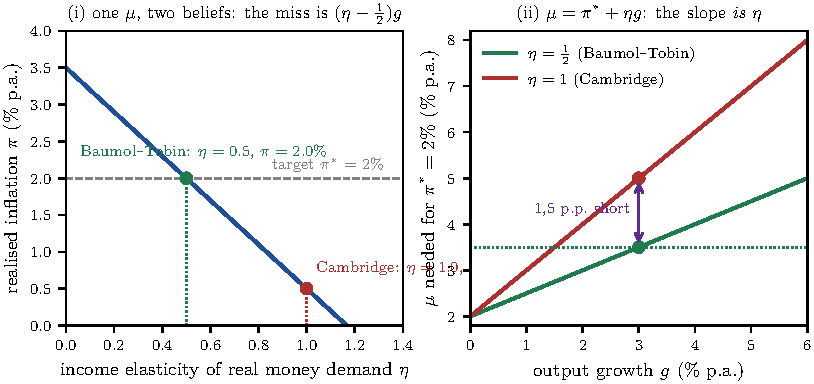
\includegraphics[width=\linewidth]{fig/fig_l6q2_eta.pdf}\\[3pt]
\captionof{figure}{Q2(b). Left: with money growth locked at $\mu=3{,}5\%$, realised inflation
$\pi=\mu-\eta g$ falls in the elasticity at rate $g$; the Baumol--Tobin belief hits the target
and the Cambridge truth delivers $0{,}5\%$. Right: the money growth the bank must announce,
$\mu=\pi^{\ast}+\eta g$ --- the \emph{slope} of each schedule is $\eta$, so the vertical gap at
$g=3\%$ is exactly the $1{,}5$ p.p.\ of \eqref{eq:erro}.}
\label{fig:eta}
\end{center}

\begin{tcolorbox}[trapbox, title={The trap: re-optimising $\mu$ after learning the truth}]
\small
Item (iii) does not ask what the bank should now do; it asks what inflation \emph{will be}
given the announced $\mu=3{,}5\%$ and the true $\eta=1$. Answering ``the bank should set
$\mu=5\%$'' answers a different question. Say the realised rate first ($0{,}5\%$), then --- if
you want the extra line --- note that the corrected rule is $\mu=\pi^{\ast}+g=5\%$.
\end{tcolorbox}

%----------------------------------------------------------------------
\subsection*{Item (c) --- a falling trip cost: $\pi=\mu-\tfrac12(g+f)$}
%----------------------------------------------------------------------

\passo{Step 1. Put $F$ back into money demand.}
Item (b) froze $F$; now it moves, at the constant rate $\dot F/F=f<0$. Take logs of
\eqref{eq:bt} keeping every argument:
\begin{equation}
\ln \md \;=\; \tfrac12\ln Y + \tfrac12\ln F - \tfrac12\ln i - \tfrac12\ln 2 .
\label{eq:lnbt}
\end{equation}

\passo{Step 2. Differentiate in time.}
With $i$ constant ($\dot\imath=0$), \eqref{eq:lnbt} gives the growth rate of real money demand
\begin{equation}
\frac{\dot{\md}}{\md} \;=\; \tfrac12\,\frac{\dot Y}{Y} + \tfrac12\,\frac{\dot F}{F}
\;=\; \resp{\tfrac12\,(g+f).}
\label{eq:mdot}
\end{equation}
This is \eqref{eq:growth} with a second shifter: the \emph{same} $\tfrac12$ applies to the
technology term as well, because Baumol--Tobin gives $F$ and $Y$ the identical exponent.

\passo{Step 3. Substitute into the growth-rate equilibrium condition.}
Market clearing in growth rates is $\mu=\pi+\dot{\md}/\md$, so
\begin{equation}
\boxed{\;\resp{\pi \;=\; \mu - \tfrac12\,(g+f)\;}}
\label{eq:pigf}
\end{equation}
which nests item (a): $f=0$ returns $\pi=\mu-\tfrac12 g$, i.e.\ $\pi=\mu-\eta g$ with
$\eta=\tfrac12$. The symmetric form $\pi=\mu-\eta(g+f)$ holds here only because
$\varepsilon_{\md,F}=\varepsilon_{\md,Y}=\tfrac12$ in this particular model.

\passo{Step 4. Cross-check through velocity.}
From \eqref{eq:velocity}, $V=\sqrt{2iY/F}$, so at constant $i$
\[
\hat V \;=\; \tfrac12\,(g-f) \;>\; 0 \quad\text{when } f<0 ,
\]
and the quantity equation in growth rates, $\mu+\hat V=\pi+g$, gives
$\pi=\mu+\tfrac12(g-f)-g=\mu-\tfrac12(g+f)$. \checkmark\ \resp{The two routes agree, which is
the point of Question 1(b): money demand and velocity are the same statement read in opposite
directions.}

\passo{Why a falling $F$ is inflationary under a constant-$\mu$ rule.}
Read \eqref{eq:pigf} as $\partial\pi/\partial f=-\tfrac12<0$: a \emph{more negative} $f$ raises
$\pi$. The economics, in three steps:
\begin{itemize}
\item \textbf{Cheaper trips mean people want to hold less cash.} ATMs, debit cards, internet
      banking and Pix all cut the fixed cost of converting interest-bearing wealth into means
      of payment. With $F$ falling, the optimal number of trips $\Nst=\sqrt{iY/2F}$ rises and
      average real balances $\md=\sqrt{YF/2i}$ fall, for given $Y$ and $i$.
\item \textbf{The rule keeps supplying money at $\mu$ regardless.} Money growth is fixed by
      the policy rule, so the supply of real balances grows at $\mu-\pi$ whatever happens to
      the demand for them. Payments innovation has shifted money demand in while the supply
      schedule kept marching out.
\item \textbf{Only the price level can clear the gap.} Nobody is forced to hold real balances
      they do not want; the excess supply is spent, and the price level rises until $\Ms/p$ is
      back down to the smaller $\md$ people now wish to hold. \resp{So the innovation is
      inflationary not because it creates money --- it creates none --- but because it
      destroys demand for money.}
\end{itemize}
With the numbers of item (b), $\mu=3{,}5\%$ and $g=3\%$, a payments technology improving at
$f=-2\%$ per year delivers $\pi=3{,}5-\tfrac12(3-2)=3\%$ instead of $2\%$: a full percentage
point of target miss, from a channel that never appears in $\pi=\mu-g$.

\begin{center}
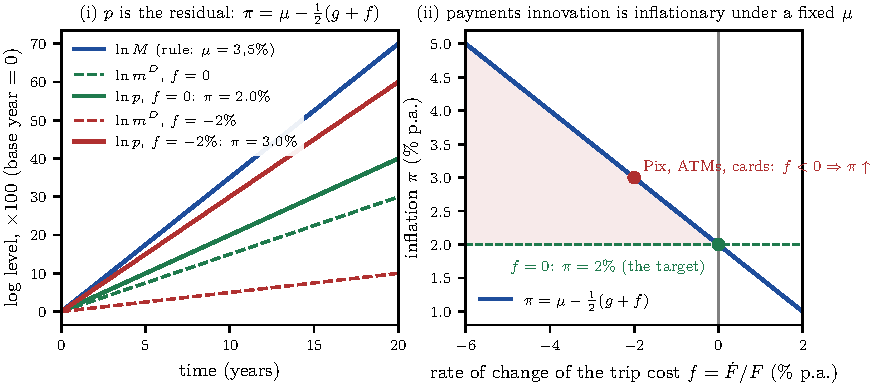
\includegraphics[width=\linewidth]{fig/fig_l6q2_trips.pdf}\\[3pt]
\captionof{figure}{Q2(c). Left: under the fixed rule $\mu=3{,}5\%$, real money demand grows at
$\tfrac12(g+f)$ and the price level is the residual; a falling $F$ flattens $\ln \md$ and
steepens $\ln p$. Right: inflation against the rate of decline of the trip cost. The shaded
wedge is the inflation a constant-$\mu$ rule delivers \emph{in excess} of its $f=0$ design
value.}
\label{fig:trips}
\end{center}

\begin{tcolorbox}[theorybox, title={The policy moral, and why the constant-money-growth rule lost}]
\small
A constant money growth rule is only as good as the stability of money demand. Equation
\eqref{eq:pigf} shows that such a rule silently assumes $f=0$ --- a frozen payments technology
--- on top of assuming a known $\eta$. In the 1980s exactly this happened: financial
innovation cut $F$, velocity drifted up, and monetary targets delivered inflation different
from what the arithmetic promised. That is the empirical reason central banks moved to the
interest-rate instrument of Question 1(d): a rate rule lets $M$ adjust endogenously to
whatever $\md$ turns out to be, so shifts in $F$ are absorbed by the money stock instead of
landing on prices. In Brazil, Pix is the textbook case of a large, fast fall in $F$.
\end{tcolorbox}

\begin{tcolorbox}[planbox, title={Interactive companions (already in this project)}]
\small
The algebra above is the static picture of three pages in \texttt{Map/}; use them to move the
parameters instead of re-plotting by hand:
\begin{itemize}
\item \texttt{Map/aula-07-moeda-inflacao/companion-inflation-rule.html} --- \emph{this
      question}: sliders on $\mu$, $g$, $\eta$, $f$ and $\pi^{\ast}$, the three panels of the
      figures above made live, and read-outs for $\pi$, the target gap, the required $\mu$ and
      the velocity drift. The $\eta$ slider steps in $0{,}01$, so $\tfrac12$ and $1$ are both
      landed on exactly.
\item \texttt{Map/aula-07-moeda-inflacao/companion-baumol-tobin.html} --- sliders on $Y$, $i$
      and $F$, with live read-outs of $\Nst$, $\md$, $V$ and both elasticities. Dragging $F$
      down is item (c); raising $Y$ and watching $V$ rise is $\eta=\tfrac12<1$.
\item \texttt{Map/aula-07-moeda-inflacao/companion-seigniorage.html} --- what the government
      collects from the $\mu$ chosen here, and the Laffer curve behind it.
\end{itemize}
The two static figures above come from \texttt{Resolucao/lista6\_codigo/l6\_figuras.py}; run it
directly to re-check the numbers --- it asserts $\mu=3{,}5\%$, $\pi=0{,}5\%$ and the velocity
cross-check of Step 4.
\end{tcolorbox}

\begin{tcolorbox}[rubricbox]
\small
\begin{itemize}
\item \textbf{(a)} Log-differentiate $\Ms=p\,\md(Y,i)$; state explicitly that $\dot\imath=0$
      kills the interest term (\emph{not} $\md_i=0$); reach $\pi=\mu-\eta g$; read it as
      ``inflation is money growth minus real money demand growth''. Bonus: $\hat V=(1-\eta)g$,
      and $\eta=1$ is the constant-velocity quantity theory.
\item \textbf{(b)} (i) $\eta=\tfrac12$, as the exponent of $Y$ in $\md=\sqrt{YF/2i}$, with the
      scale-economy reading. (ii) $\mu=\pi^{\ast}+\eta g=3{,}5\%$. (iii) $\pi=3{,}5-3=0{,}5\%$,
      an undershoot of $1{,}5$ p.p.\ $=(\eta^{\text{true}}-\eta^{\text{assumed}})g$; do not
      re-optimise $\mu$ instead of answering the question asked.
\item \textbf{(c)} $\ln\md=\tfrac12\ln Y+\tfrac12\ln F+\text{const}$ at constant $i$
      $\Rightarrow$ $\dot{\md}/\md=\tfrac12(g+f)$ $\Rightarrow$ $\pi=\mu-\tfrac12(g+f)$;
      cross-check via $\hat V=\tfrac12(g-f)$. The explanation must say that falling $F$
      \emph{reduces the demand} for real balances, so a fixed $\mu$ becomes excessive and $p$
      clears the market --- and, ideally, connect it to the failure of monetary targeting.
\end{itemize}
\end{tcolorbox}

\end{document}
